% Supplementary Information. All numbers come from ../data_v3 (generated by ../src_v3).
\documentclass[11pt]{article}
\usepackage[utf8]{inputenc}
\usepackage[T1]{fontenc}
\usepackage{amsmath,amssymb}
\IfFileExists{mathdesign.sty}{\usepackage[bitstream-charter]{mathdesign}}{\usepackage{lmodern}}
\usepackage{booktabs}
\usepackage{graphicx}
\usepackage[section]{placeins}
\usepackage[margin=1in]{geometry}
\usepackage{xcolor}
\providecommand{\ohmcm}{\ensuremath{\Omega\cdot\mathrm{cm}}}
\providecommand{\ohmum}{\ensuremath{\Omega\cdot\mu\mathrm{m}}}
\usepackage{xr-hyper}
\usepackage[colorlinks,linkcolor={red!50!black},citecolor={blue!50!black},urlcolor={blue!80!black}]{hyperref}
\externaldocument[M-]{InSe_v3}
\usepackage[english]{babel}
\urlstyle{same}
\providecommand{\doi}[1]{\href{https://doi.org/#1}{doi:\,#1}}
\DeclareSymbolFont{usualmathcal}{OMS}{cmsy}{m}{n}
\DeclareSymbolFontAlphabet{\mathcal}{usualmathcal}
\graphicspath{{../figures_v3/}}
\providecommand{\ohmcm}{\ensuremath{\Omega\cdot\mathrm{cm}}}
\providecommand{\ohmum}{\ensuremath{\Omega\cdot\mu\mathrm{m}}}
\renewcommand{\thesection}{S\arabic{section}}
\renewcommand{\thefigure}{S\arabic{figure}}
\renewcommand{\thetable}{S\arabic{table}}
\renewcommand{\theequation}{S\arabic{equation}}
\sloppy

\title{Supplementary Information for\\ ``Which Contact Geometry for p-Type InSe? Pinning, Barrier Height and Hole-Mass Anisotropy in an Electro-Thermal Device Simulation''}
\author{Harsha Adhikary \\[4pt] \small Department of Physics, Indian Institute of Science (IISc), Bengaluru, India}
\date{}

\begin{document}
\maketitle
\noindent Section, figure and table numbers without an ``S'' refer to the main text.

\section{Verification}
\label{sec:ver}
Table~\ref{tab:ver} and Fig.~\ref{fig:ver} summarise nine tests: (V1) an ohmic resistor; (V2) a finite-velocity contact resistor; (V3) Mott--Gurney space-charge-limited current with Boltzmann and Fermi--Dirac statistics \cite{simott}; (V4) thermionic emission at 300 and 350~K; (V5) energy and charge conservation in 2D, gated and ungated (heat out equals $IV$ within 0.3\% except 1.2\% in the hottest gated case, where Thomson heat from temperature gradients is not separately balanced); (V6) nonlocal tunnelling against an independent quadrature on the same band profile (0.17\%), and on a depletion-approximation profile (13\%, the approximation's own error); (V7) a degenerate contact at equilibrium; (V8) transient energy conservation and approach to the DC state; and (V9) Gauss's law with a gate. $R_{\rm tot}$ changes by less than 1.3\% between 0.5$\times$ and 3$\times$ mesh density in the ungated device (\texttt{data\_v3/mesh\_ungated.csv}), and by at most 1.5\% (with $\Delta T_{\max}$ changing by at most 0.6~K) at the operating points of Table~\ref{M-tab:therm} between 1$\times$ and 3$\times$. Convergence is slower in the tunnelling-dominated on state at the measured pinning: between 1$\times$ and 3$\times$ the edge-contact resistance changes non-monotonically by up to 12\% and the top-contact resistance by up to 5\% (Fig.~\ref{fig:electron}c). On-state resistances and top/edge ratios there carry a mesh uncertainty of about 15\%.

\begin{table}[!htbp]
\centering
\caption{Verification summary (\texttt{data\_v3/verification\_summary.csv}).}
\label{tab:ver}\small
\begin{tabular}{@{}lp{0.7\textwidth}r@{}}
\toprule
Test & Quantity & Relative error \\
\midrule
V1 & R ohmic (Ohm cm\^{}2) & +1.9e-14 \\
V2 & R Robin v=1e+09 (Ohm cm\^{}2) & +4.5e-10 \\
V2 & R Robin v=1e+05 (Ohm cm\^{}2) & +4.5e-05 \\
V2 & R Robin v=1e+04 (Ohm cm\^{}2) & +1.2e-03 \\
V3 & boltzmann J/J\_MG at 160 V & +7.5e-03 \\
V3 & fd J/J\_MG at 160 V & -5.5e-03 \\
V4 & ideality (300 K) & -6.3e-03 \\
V4 & $|$J\_rev(0.3V)$|$ (300 K) & -1.2e-03 \\
V4 & ideality (350 K) & -9.4e-03 \\
V4 & $|$J\_rev(0.3V)$|$ (350 K) & -1.4e-03 \\
V5 & top 4.8eV 0.05V P\_out/IV & -2.7e-04 \\
V5 & top 4.8eV 0.05V -I\_src/I\_drn & +1.3e-14 \\
V5 & top 5.0eV 0.5V P\_out/IV & +2.7e-04 \\
V5 & top 5.0eV 0.5V -I\_src/I\_drn & -2.8e-14 \\
V5 & top-gated 4.8eV 0.05V P\_out/IV & -4.7e-04 \\
V5 & top-gated 4.8eV 0.05V -I\_src/I\_drn & +0.0e+00 \\
V5 & top-gated 5.0eV 0.5V P\_out/IV & +2.3e-03 \\
V5 & top-gated 5.0eV 0.5V -I\_src/I\_drn & +5.4e-15 \\
V5 & edge 4.8eV 0.05V P\_out/IV & +1.4e-03 \\
V5 & edge 4.8eV 0.05V -I\_src/I\_drn & -1.8e-14 \\
V5 & edge 5.0eV 0.5V P\_out/IV & +2.9e-03 \\
V5 & edge 5.0eV 0.5V -I\_src/I\_drn & +4.4e-16 \\
V5 & edge-gated 4.8eV 0.05V P\_out/IV & +7.5e-04 \\
V5 & edge-gated 4.8eV 0.05V -I\_src/I\_drn & -1.8e-16 \\
V5 & edge-gated 5.0eV 0.5V P\_out/IV & +1.2e-02 \\
V5 & edge-gated 5.0eV 0.5V -I\_src/I\_drn & +2.0e-15 \\
V6 & J\_tun: model vs quad on same profile & -1.7e-03 \\
V6 & J\_tun: model vs depletion-approximation quadrature (approximation difference) & -1.3e-01 \\
V7 & p\_s / (N\_V F1/2(-phiB/kT)) [exact F] & -4.7e-04 \\
V7 & $|$I(V=0)$|$ (A/cm\^{}2) & 4.8e-07 (abs.) \\
V7 & max$|$phi\_p$|$ at equilibrium (V) & 1.7e-04 (abs.) \\
V8 & (E\_out + E\_stored)/E\_in (0-1 us) & -4.2e-04 \\
V8 & T\_max(1 us) - 300 vs DC & +0.0e+00 \\
V9 & (sum contact charge + semi charge)/$|$Q\_gate$|$ & -2.5e-06 \\
\\
\bottomrule
\end{tabular}
\end{table}

\begin{figure}[!htbp]
\centering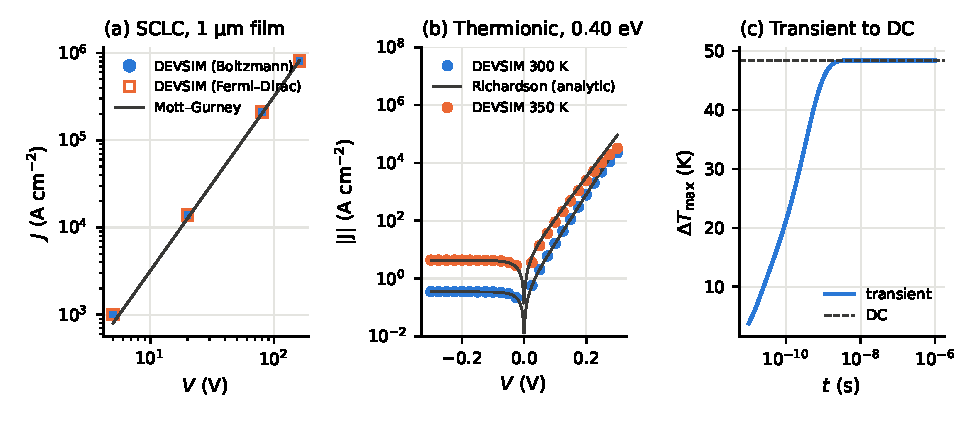
\includegraphics[width=0.96\textwidth]{fig1_verification.pdf}
\caption{Verification. (a) Mott--Gurney law with Boltzmann and Fermi--Dirac statistics. (b) Thermionic emission at 300 and 350~K. (c) Transient heating of a gated edge device stepped to 1~V (tunnelling off), approaching the DC solution.}
\label{fig:ver}
\end{figure}

\section{Numerical benchmark on Au/MoS$_2$}
\label{sec:cal}
The benchmark uses ultra-high-vacuum Au on 4.5-nm MoS$_2$ with a 90-nm SiO$_2$ back gate \cite{sienglish}. The measured quantities at $n=10^{13}$~cm$^{-2}$ are $R_c=740$~\ohmum, $\rho_c\approx3\times10^{-7}$~$\Omega$\,cm$^2$ and $L_T\approx35$--40~nm at 300~K, and $\rho_c\approx1.5\times10^{-7}$~$\Omega$\,cm$^2$ and $L_T\approx20$~nm at 400~K. We keep the 0.15-eV electron barrier assumed in that work and use literature MoS$_2$ parameters, with an under-contact mobility of 35~cm$^2$/Vs scaling as $T^{-1.6}$. We fit a single parameter, $\mathcal{T}_{\rm vdW}$, to $R_c(300\,{\rm K})$ only. The quantities predicted out of sample are $L_T(300\,\rm K)$ (from simulated $R_c(L_c)$ with $L_c=20$--200~nm), and $\rho_c$ and $L_T$ at 400~K.

The fit gives $\mathcal{T}_{\rm vdW}=1.0$, at its physical bound: $R_c=731$~\ohmum\ against 740~\ohmum\ measured. With the literature barrier, nonlocal tunnelling carries 99.8\% of the injection, and no additional vdW tunnel barrier is needed. Without further adjustment the model gives $L_T=34$~nm and $\rho_c=2.7\times10^{-7}$~$\Omega$\,cm$^2$ at 300~K: $\rho_c$ lies within the measured range, and $L_T$ is 3\% below the lower end of the measured 35--40~nm. At 400~K it predicts $\rho_c=2.0\times10^{-7}$~$\Omega$\,cm$^2$ (measured 1.5) and $L_T=29$~nm (measured $\approx$20, quoted uncertainty up to 50\%), with the measured direction of change for both (Fig.~\ref{fig:mos2}). The model underestimates how much $L_T$ shrinks with temperature, consistent with its temperature-independent barrier and the absence of phonon-assisted injection. Ref.~\cite{sienglish} attributes the fall of $\rho_c$ with temperature to thermionic emission, whereas the model assigns the injection almost entirely to tunnelling, so the agreement validates the numerics rather than the mechanism. MoS$_2$ has a different band structure, no strong anisotropy and no layer-dependent gap, so the benchmark does not validate the InSe parameters.

\begin{figure}[!htbp]
\centering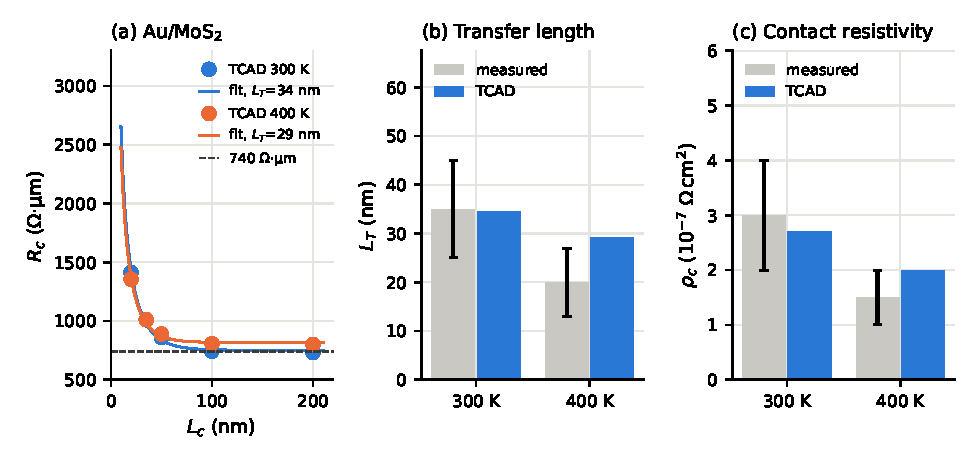
\includegraphics[width=0.96\textwidth]{fig8_mos2_calibration.pdf}
\caption{(a) Simulated $R_c(L_c)$ of Au/MoS$_2$ at 300 and 400~K with transmission-line fits. (b) Transfer length and (c) specific contact resistivity against the measurements of Ref.~\cite{sienglish}, with their quoted uncertainties. Only $R_c$ at 300~K was fitted; the 400~K values and $L_T$ are predictions.}
\label{fig:mos2}
\end{figure}

\section{Ungated InSe: work function, statistics, tunnelling and anisotropy}
\label{sec:ungated}
Without a gate (Fig.~\ref{fig:wf}), $R_{\rm tot}$ at 0.05~V falls exponentially with $\Phi_M$ down to $E_V=5.0$~eV. For 4.8~eV it is 1430~\ohmcm\ (edge), 5080~\ohmcm\ (top, 50~nm) and 11\,500~\ohmcm\ (top, 10~nm). With Fermi--Dirac statistics the resistance keeps decreasing for degenerate contacts: at 5.65~eV it is 5.4, 7.3 and 7.7~\ohmcm, a factor 2.1--2.6 below the Boltzmann result, which is clipped at $E_V$. Contacts carry 67\% (top, 50~nm) and 87\% (top, 10~nm) of $R_{\rm tot}$ at 4.8~eV, against 7.5\% for the edge. In the ungated, fully depleted film, nonlocal tunnelling carries 44\% of the edge-contact current and lowers its resistance by 13\% relative to pure thermionic emission. For top contacts it carries $\leq$8.5\% and lowers resistance by 2--6\%. For the edge contact the local $\Gamma(F)$ model recovers only a fifth of this reduction (2.3\% vs 12.6\%), because only nonlocal injection bypasses the diffusion-limited part of the barrier; for top contacts, where injection is limited by the interface, the two models differ by about 1\%.

Out-of-plane transport limits top contacts (Fig.~\ref{fig:aniso}). Lowering $\mu_\perp/\mu_\parallel$ from 1 to 0.002 doubles the top-contact resistance at 4.8~eV (3920$\to$7990~\ohmcm\ for 50~nm; 8270$\to$16\,700~\ohmcm\ for 10~nm), whereas edge contacts are unaffected. The edge advantage at 4.8~eV therefore grows from 64\% (isotropic) to 72\% (baseline) and 82\% ($r_\mu=0.002$). The top-contact resistance saturates for $L_c\gtrsim50$--100~nm. Thermal anisotropy matters little at this thickness: with $\kappa_\perp=0.76$ instead of 8.5~W/mK, the temperature rise of ungated devices at 1~V changes by less than 4\% (the gated operating point is more sensitive: 8--17\%).

\begin{figure}[!htbp]
\centering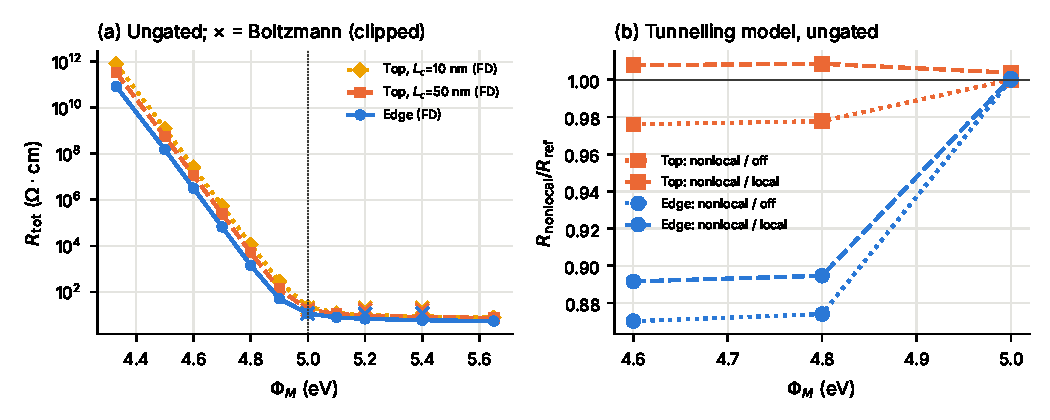
\includegraphics[width=0.96\textwidth]{fig3_wf_statistics_tunnelling.pdf}
\caption{Ungated devices. (a) $R_{\rm tot}$ versus $\Phi_M$ with Fermi--Dirac statistics (lines) and Boltzmann statistics clipped at $E_V$ ($\times$). (b) Ratio of nonlocal-tunnelling resistance to the no-tunnelling and local-$\Gamma$ models.}
\label{fig:wf}
\end{figure}

\begin{figure}[!htbp]
\centering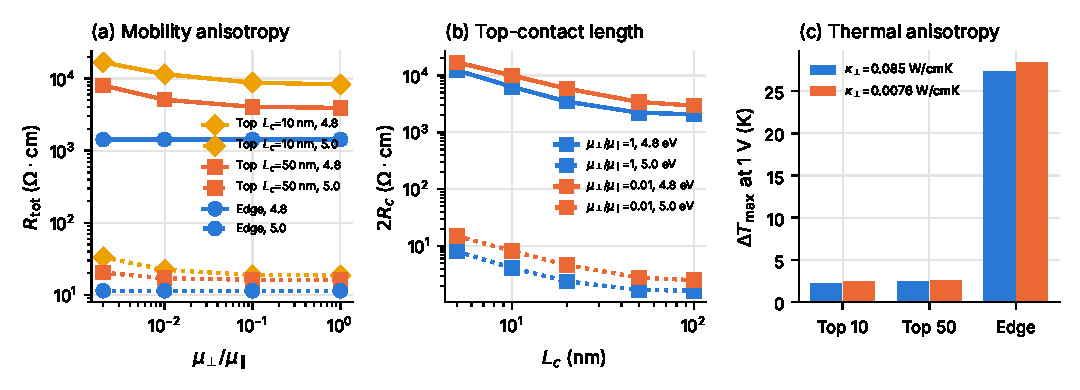
\includegraphics[width=0.96\textwidth]{fig4_anisotropy.pdf}
\caption{(a) $R_{\rm tot}$ versus out-of-plane/in-plane mobility ratio (colour: geometry; line style: $\Phi_M$). (b) $2R_c$ of top contacts versus contact length for two mobility ratios. (c) Peak temperature rise of ungated devices at 1~V for isotropic and measured $\kappa_\perp$.}
\label{fig:aniso}
\end{figure}

\section{Electron injection with the measured pinning, and mesh convergence}
\label{sec:electron}
As a consistency check against the measured electron barriers, we applied the model to electron injection into an n-type film ($N_D=10^{16}$~cm$^{-3}$) with the measured direct pinning, for In, Ti and Pd contacts at 200--400~K (Fig.~\ref{fig:electron}a,b). At $V_G=0$ the Arrhenius barriers, from the slope of $\ln(I/T^2)$ against $1/T$, are 0.14--0.17~eV (edge) and 0.20--0.24~eV (top). They differ by at most 0.04~eV between metals across a 1-eV range of work function, in line with the weak metal dependence reported in Ref.~\cite{sichen}. They lie 0.06--0.16~eV below the input barrier of 0.30~eV because tunnelling contributes even without a gate, so barriers extracted this way are lower bounds. Above $V_G=+1$~V the Arrhenius slope turns negative because channel transport dominates. Figure~\ref{fig:electron}c shows the mesh convergence of the on-state resistances quoted in Sec.~\ref{M-sec:measured}.

\begin{figure}[!htbp]
\centering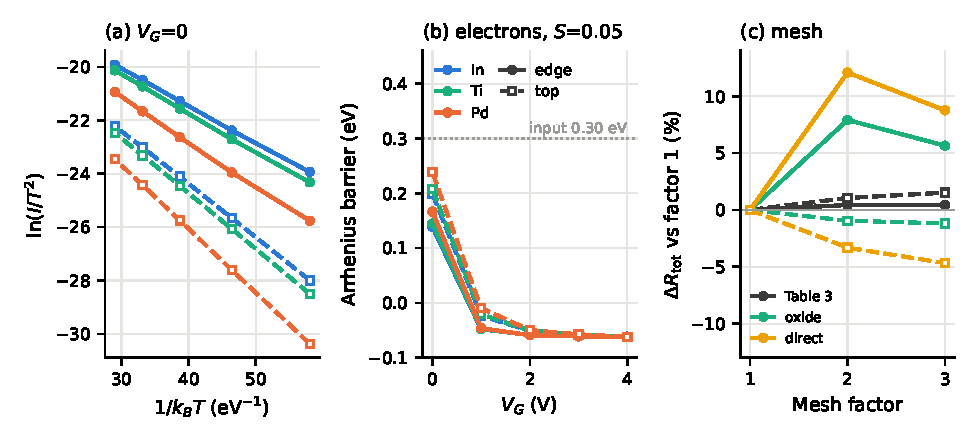
\includegraphics[width=0.96\textwidth]{fig15_electron_mesh.pdf}
\caption{(a) Arrhenius plots of electron injection at $V_G=0$ with the measured direct pinning ($S=0.05$, input barrier 0.30~eV) for In, Ti and Pd; filled: edge, open: top. (b) Arrhenius barrier versus $V_G$. (c) Change of $R_{\rm tot}$ with mesh factor for the operating point of Table~\ref{M-tab:therm} and for the gated on state at the measured pinning (Pt, $V_G=-3$~V).}
\label{fig:electron}
\end{figure}

\section{Thickness and self-heating at the measured alignment}
\label{sec:thickalign}
Figure~\ref{fig:measuredalign} repeats the thickness and thermal analyses at the literature alignment. With Pt contacts ($V_G=-3$~V) edge contacts improve monotonically from 3 to 12 layers (oxide interlayer: 25$\to$4.5~\ohmcm), and top contacts have an optimum at five layers (interlayer, 207~\ohmcm) or six layers (direct pinning). At the reference alignment, changing the valence-band share of the confinement shift to 0.2 or 0.5 moves the top-contact optimum between four and five layers (Fig.~\ref{fig:measuredalign}c). Panel (a) gives the temperature rises at the measured alignment quoted in Sec.~\ref{M-sec:heat}.

\begin{figure}[!htbp]
\centering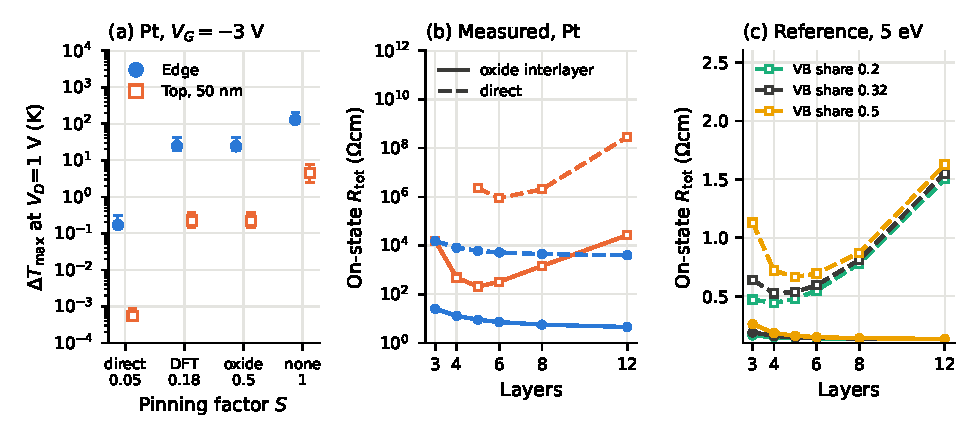
\includegraphics[width=0.96\textwidth]{fig14_measured_alignment.pdf}
\caption{Measured alignment. (a) Peak temperature rise at $V_D=1$~V, $V_G=-3$~V for Pt contacts and four pinning cases; bars span heat sinking through the metal (lower) and a three times larger $R_{\rm TBR}$ (upper). (b) On-state $R_{\rm tot}$ versus layer number for Pt with the oxide interlayer and direct pinning (missing top points did not converge). (c) Reference alignment ($\Phi_M=5.0$~eV, $S=1$) for valence-band shares of 0.2, 0.32 and 0.5. Filled: edge; open: top, 50~nm.}
\label{fig:measuredalign}
\end{figure}

\section{Heat distribution and heat-model terms}
\label{sec:heatterms}
The two-dimensional maps in Fig.~\ref{fig:maps} show where the heat sits: in the top-contacted device the hottest point lies at the drain-side channel end on the contact side of the film, and the whole film stays within 24~K of ambient; in the edge-contacted device the film is 126--150~K hot everywhere and is coolest at the oxide interface, through which heat leaves to the substrate. At the operating points of Table~\ref{M-tab:therm} the heat leaving the device equals $IV$ within 0.5\% (top) and 1.2--1.9\% (edge, 0.5 and 1~V). For the 150~K edge rise this is about 3~K, larger than the Peltier effect, so temperatures are quoted to $\pm3$~K.

The individual heat terms (Fig.~\ref{M-fig:thermal}b) change $\Delta T_{\max}$ as follows. Using bulk Joule heat only underestimates $\Delta T_{\max}$ by 7--8\% and misses 8--15\% of the dissipated power. The measured out-of-plane conductivity, compared with isotropic $\kappa$, raises $\Delta T_{\max}$ by 8\% (edge) and 17\% (top). Heat sinking through the metal contacts lowers it by 23\% (edge) and 42\% (top). A ten times smaller thermal boundary resistance at the gate lowers it by 35--37\%, and a three times larger one raises it by 58--73\%. Peltier heat cools the hole-injecting contact and heats the collecting one (top, 1~V: source $+11.9$~K, drain $+21.6$~K with Peltier, against $+13.5$ and $+20.9$~K without). Temperature-dependent statistics change temperatures by less than 1\%. After a drain step simulated without tunnelling (Fig.~\ref{M-fig:thermal}c), 63\% of the final rise is reached at 0.20~ns (top) and 0.25~ns (edge). To include tunnelling, we also found the electrical state at fixed bias with all heat sources off and then switched them on at $t=0$, integrating the heat equation with the tunnelling sources frozen at their initial values (\texttt{data\_v3/heat\_step.csv}). At the operating point of Table~\ref{M-tab:therm} (1~V) the final rises are 156~K (edge) and 24~K (top), and 63\% is reached at 0.19 and 0.22~ns; without tunnelling the same protocol gives 0.25 and 0.21~ns. For unpinned Pt contacts at the measured alignment ($V_G=-3$~V, 1~V) the edge device heats by 149~K with 0.20~ns, and the top device by 4.4~K with 0.22~ns. The time constant is therefore set by the heat path, not by the injection mechanism.

The contact Peltier term uses $J_sT(k/q)(c-\eta_s)$ with the thermionic constant $c=2$. The Scharfetter--Gummel flux with a mobility independent of carrier energy implies $c=3/2$, so the two are consistent only to within $kT/2$ per carrier. Rerunning the operating points of Table~\ref{M-tab:therm} with $c=3/2$ (\texttt{data\_v3/thermo\_const.csv}) changes $\Delta T_{\max}$ by $-3.3$~K (edge, 1~V), $-0.1$~K (edge, 0.5~V) and less than 0.1~K (top). The energy-balance residual becomes $-0.3$\% and $+0.5$\% for the edge device (from $+1.2$\% and $+1.9$\%) and $-2.1$\% and $-0.8$\% for the top device (from $+0.2$\% and $+0.5$\%).

\begin{figure}[!htbp]
\centering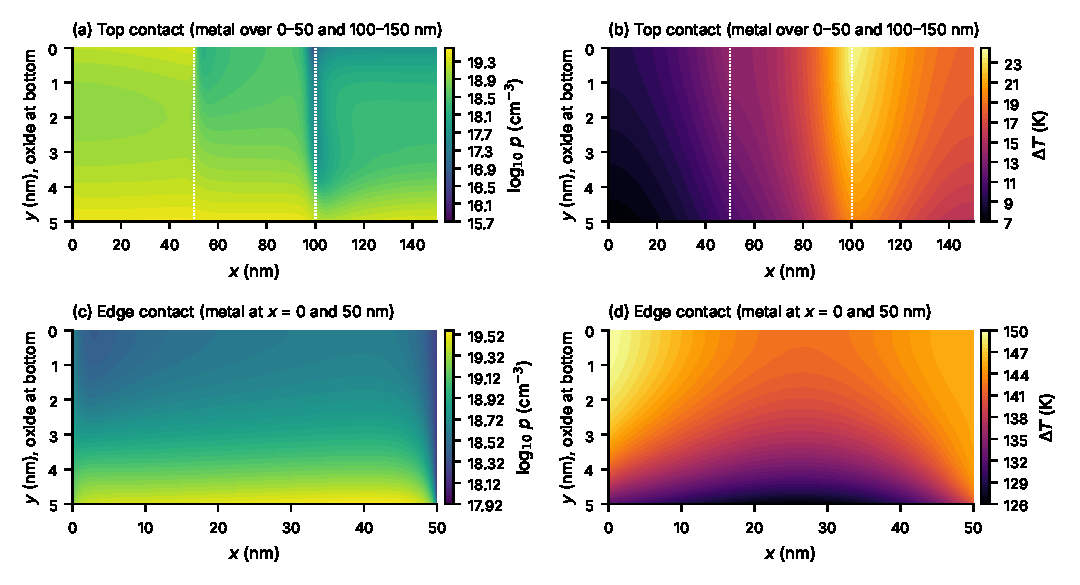
\includegraphics[width=0.96\textwidth]{fig11_field_maps.pdf}
\caption{Hole density and temperature rise of gated devices at $V_D=1$~V, $V_G=-2$~V, $\Phi_M=5.0$~eV (full model). The vertical axis is stretched: the film is 5~nm thick. The oxide interface is at the bottom ($y=5$~nm). Dotted lines in (a, b) mark the channel ends.}
\label{fig:maps}
\end{figure}

\section{Compact model}
\label{sec:compact}
For top contacts in the barrier-limited regime we compare a transmission-line model with the simulation. The model uses an interface resistivity $\rho_{\rm if}=V_t/(qv_R\mathcal{T}_{\rm vdW}p_{\rm eq})$, a vertical access term $t/(2q\mu_\perp\bar p)$, an under-contact sheet resistance $1/(q\mu_\parallel\bar pt)$, and $R_c=\sqrt{\rho R_{\rm sh}}\coth(L_c/L_T)$. Over 120 cases ($\phi_{Bp}=0.05$--0.25~eV, $d_{\rm vdW}=0.2$--0.4~nm, $L_c=10$--100~nm, $r_\mu=1$ and 0.01) the fully predictive version, with $\bar p=p_{\rm eq}$, has a median error of 11\% and a 90th-percentile error of 33\% (Fig.~\ref{fig:compact}). Taking $\bar p$ from the simulation reduces the 90th percentile to 20\%. The compact model is therefore adequate for circuit-level estimates when tunnelling is weak, that is, without strong gating.

\begin{figure}[!htbp]
\centering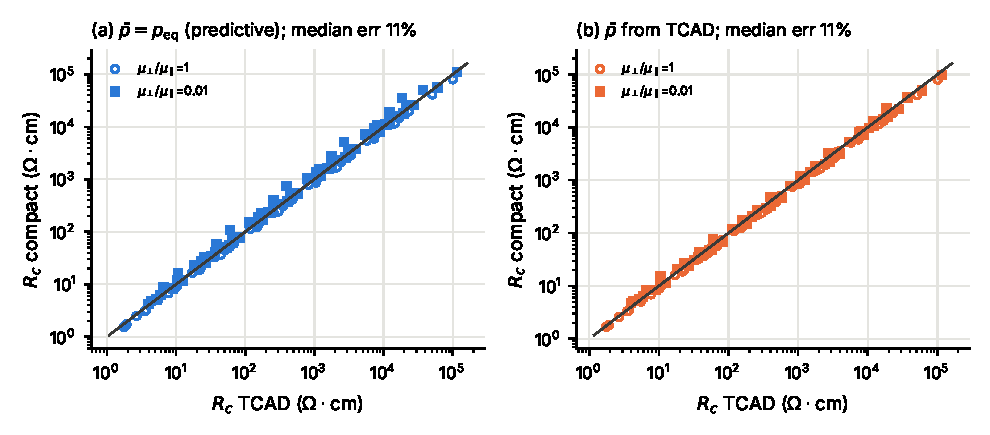
\includegraphics[width=0.96\textwidth]{fig9_compact_model.pdf}
\caption{Compact transmission-line model against simulated top-contact $R_c$ (no tunnelling), with (a) $\bar p=p_{\rm eq}$ and (b) $\bar p$ from the simulation.}
\label{fig:compact}
\end{figure}

\section{Ungated Monte Carlo analysis}
\label{sec:uq}
We propagated the uncertainty of the least-known inputs for ungated devices at the reference alignment: 120 samples, each simulated for both geometries at 4.8 and 5.0~eV, at 0.05~V. The sampling ranges were $\Delta E_V\sim\mathcal N(0,0.1~\mathrm{eV})$ and $S\sim U(0.3,1)$, the same for both contacts; $d_{\rm vdW}\sim U(0.2,0.4)$~nm and $\Phi_{\rm vdW}\sim U(1,3)$~eV; log-uniform $\mu_p$ (20--100~cm$^2$/Vs), $\mu_\perp/\mu_\parallel$ (0.002--0.1) and $N_A$ ($10^{15}$--$10^{17}$~cm$^{-3}$); $\varepsilon_r\sim U(5,8)$ and $m_h\sim U(0.1,0.3)$. The resulting 5--95\% range of $R_{\rm tot}$ spans seven to eight orders of magnitude: 61--$1.2\times10^9$~\ohmcm\ for the edge contact at 4.8~eV (Fig.~\ref{fig:uq}a). The band alignment ($\Delta E_V$, Spearman $\rho=-0.63$ to $-0.77$) and the pinning factor ($\rho=-0.69$ to $-0.81$) account for nearly all of the variance. Their first-order indices are 0.47--0.77, while all other parameters stay at or near the estimator's noise floor of about 0.06--0.17 for $n=120$ (Fig.~\ref{fig:uq}c). When both contacts share the same pinning, the edge contact has lower resistance in every sample. The edge/top ratio has a median of 0.24, with a 5--95\% range of 0.07--0.51 at 4.8~eV and 0.08--0.72 at 5.0~eV. This analysis excludes the measured $S=0.05$ and uses a spread of $\Delta E_V$ smaller than the difference between the reference, calculated and measured alignments, which is why the main text repeats it for the gated on state at the literature alignment.

\begin{figure}[!htbp]
\centering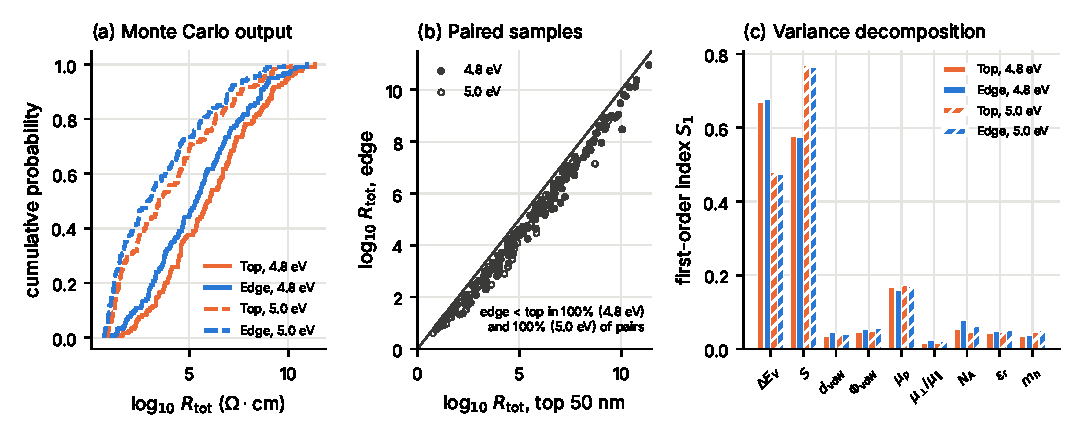
\includegraphics[width=0.96\textwidth]{fig10_uncertainty.pdf}
\caption{Monte Carlo propagation of parameter uncertainty (ungated, 0.05~V). (a) Cumulative distributions of $\log_{10}R_{\rm tot}$. (b) Paired samples: the same parameter draw simulated for the top (50~nm) and edge contact; points below the diagonal have lower edge resistance. (c) First-order variance indices (colour: geometry; hatching: 5.0~eV). Indices below about 0.06--0.17 are within the noise floor of the estimator for $n=120$ (permutation test).}
\label{fig:uq}
\end{figure}

\section{Tunnelling direction}
\label{sec:oblique}
By default each contact node tunnels along the inward normal: vertically for top contacts and in-plane for edge contacts. As a test, every node of an edge contact, and every node of a top contact within 15~nm of its channel-side edge, instead considered straight paths at 0, 15, 30, 45, 60 and 75$^\circ$ from the normal on both sides, traced through the nearest grid nodes, and used the one with the largest supply-weighted transmission (\texttt{data\_v3/oblique.csv}). Table~\ref{tab:oblique} compares both treatments in the gated on state with the light isotropic mass. Oblique paths lower the top-contact resistance by up to 2.4$\times$ at high barriers and the edge-contact resistance by 6--31\%, so the top/edge ratio changes by less than a factor of two in every case.

\begin{table}[!htbp]
\centering
\caption{On-state $R_{\rm tot}$ (\ohmcm; literature alignment, $V_G=-3$~V, $V_D=0.05$~V, $m_h=0.17~m_0$) with tunnelling along the contact normal and along the minimum-action straight path.}
\label{tab:oblique}\small
\begin{tabular}{lrrrrrr}
\toprule
 & \multicolumn{3}{c}{Normal path} & \multicolumn{3}{c}{Minimum-action path} \\
Case & Edge & Top & Top/edge & Edge & Top & Top/edge \\
\midrule
$\phi_{Bp}=0.2$~eV & 0.342 & 4.77 & 14.0 & 0.321 & 4.75 & 14.8 \\
$\phi_{Bp}=0.6$~eV & 17.8 & 918 & 51.5 & 12.4 & 872 & 70.4 \\
$\phi_{Bp}=1.0$~eV & 2720 & $4.18\times10^5$ & 154 & 2160 & $2.10\times10^5$ & 97.2 \\
Pt, interlayer & 7.20 & 330 & 45.9 & 5.00 & 319 & 63.8 \\
Pt, direct & 5200 & $8.84\times10^5$ & 170 & 4150 & $3.72\times10^5$ & 89.6 \\
\bottomrule
\end{tabular}
\end{table}

\section{Hole mass}
\label{sec:mass}
Table~\ref{tab:mass} gives the on-state resistances for Pt contacts with heavier hole masses (\texttt{data\_v3/mh\_sweep.csv}, \texttt{data\_v3/mh\_dir\_map.csv}). With the same mass for both geometries, a heavier mass widens the edge advantage. With direction-dependent masses (top: 0.17~$m_0$ for tunnelling; edge: $m_\parallel$ for tunnelling; density of states $m_\parallel$ for both) top contacts win at high barriers. Changing only the tunnelling mass, with the density-of-states mass kept at 0.17~$m_0$, gives top/edge ratios within a factor of 1.6 of those obtained by changing both, so the tunnelling mass is the main effect. Three directly pinned top-contact runs with isotropic masses of 1--2~$m_0$ did not converge.

\begin{table}[!htbp]
\centering
\caption{On-state $R_{\rm tot}$ (\ohmcm) of Pt contacts ($V_G=-3$~V, $V_D=0.05$~V) for isotropic and direction-dependent hole masses. --: not converged.}
\label{tab:mass}\small
\begin{tabular}{llrrr}
\toprule
Pinning & Masses & Edge & Top & Top/edge \\
\midrule
Direct & 0.17 isotropic & 5200 & $8.84\times10^5$ & 170 \\
 & 0.5 isotropic & $2.99\times10^6$ & $2.00\times10^9$ & 667 \\
 & 1.0 isotropic & $2.35\times10^8$ & $4.20\times10^{11}$ & 1790 \\
 & $m_\parallel=0.5$, dir. & $2.99\times10^6$ & $7.73\times10^5$ & 0.26 \\
 & $m_\parallel=0.9$, dir. & $1.25\times10^8$ & $6.95\times10^5$ & 0.0056 \\
Interlayer & 0.17 isotropic & 7.20 & 330 & 45.9 \\
 & 1.0 isotropic & 560 & $4.21\times10^5$ & 752 \\
 & $m_\parallel=0.5$, dir. & 84.9 & 304 & 3.58 \\
 & $m_\parallel=0.9$, dir. & 420 & 288 & 0.69 \\
Unpinned & 0.17 isotropic & 0.504 & 9.52 & 18.9 \\
 & 1.0 isotropic & 1.79 & 176 & 98.1 \\
 & $m_\parallel=0.5$, dir. & 1.01 & 9.46 & 9.39 \\
 & $m_\parallel=0.9$, dir. & 1.64 & 8.95 & 5.47 \\
\bottomrule
\end{tabular}
\end{table}

\section{Gated Monte Carlo analysis with the light isotropic hole mass}
\label{sec:uqgated}
With the light isotropic baseline mass we propagated the uncertainty of the least-known inputs by Monte Carlo sampling at the literature alignment (Pt, $V_G=-3$~V, $V_D=0.05$~V; 240 samples; Fig.~\ref{fig:uqgated}): $\Delta E_V\sim\mathcal N(0,0.3~\mathrm{eV})$; log-uniform $S$ from 0.05 to 0.5; a pinning level 0.1--0.6~eV below $E_C$; $d_{\rm vdW}\sim U(0.2,0.4)$~nm and $\Phi_{\rm vdW}\sim U(1,3)$~eV; log-uniform $\mu_p$ (20--100~cm$^2$/Vs), $\mu_\perp/\mu_\parallel$ (0.002--0.1) and $N_A$ ($10^{15}$--$10^{17}$~cm$^{-3}$); $\varepsilon_r\sim U(5,8)$ and $m_h\sim U(0.1,0.3)$. Tunnelling carries essentially all of the current in every sample. The 5--95\% range of $R_{\rm tot}$ is $10^{1.3}$--$10^{4.9}$~\ohmcm\ for the edge contact and $10^{2.7}$--$10^{7.3}$~\ohmcm\ for the top contact. The dominant inputs are the pinning level (first-order index 0.29--0.39), the hole tunnelling mass (0.25--0.27) and $S$ (0.18--0.22), against a noise floor of about 0.03. The band alignment falls to 0.06--0.07, because the pinning level is referenced to the band edges, as in the measurements. The vdW-gap parameters matter only for top contacts (Spearman $\rho\approx0.2$). With shared pinning the edge contact has lower resistance in all 233 converged samples, with a median edge/top ratio of 0.0095 (5--95\%: 0.0012--0.065); seven top-contact runs did not converge, all at strong pinning and high barrier, where the top resistance is likely to be largest. When $S_{\rm edge}$ is sampled independently of $S_{\rm top}$, the edge contact still has the lower resistance in 96\% of samples. These fractions describe the sampled ranges, not a probability for real devices. With this light mass the geometric advantage in the gated on state is therefore robust to the pinning uncertainty that decides the ungated comparison; Sec.~\ref{M-sec:pin} shows that it is not robust to the in-plane hole mass. The same analysis for ungated devices at the reference alignment (Section~\ref{sec:uq}) gives the edge contact the lower resistance in every sample with shared pinning.

\begin{figure}[!htbp]
\centering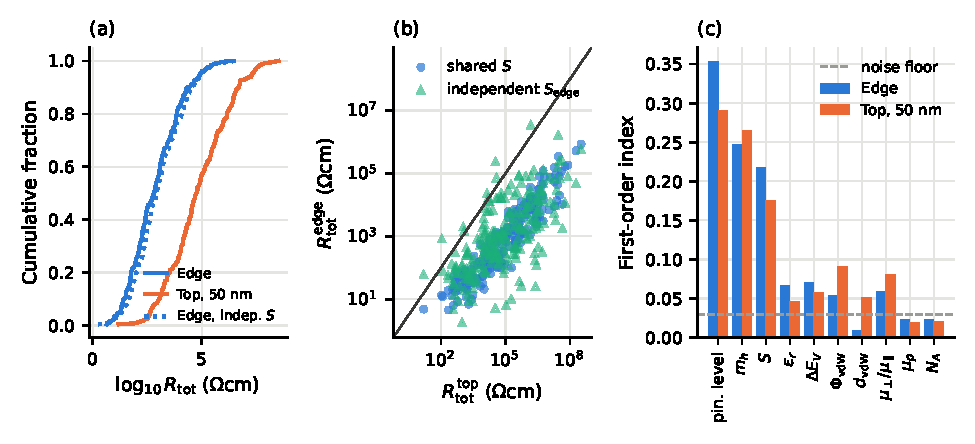
\includegraphics[width=0.96\textwidth]{fig13_uq_gated.pdf}
\caption{Monte Carlo analysis of the gated on state at the literature alignment (Pt, $V_G=-3$~V, $V_D=0.05$~V, 240 samples). (a) Cumulative distributions of $\log_{10}R_{\rm tot}$. (b) Paired samples with shared $S$ and with independently sampled $S_{\rm edge}$; points below the diagonal have lower edge resistance. (c) Binned first-order indices with the permutation noise floor.}
\label{fig:uqgated}
\end{figure}

The direction-dependent analysis of Sec.~\ref{M-sec:pin} (\texttt{data\_v3/uq\_dir.csv}) uses the same 240 samples, drawn with the same seed, and adds an in-plane mass, log-uniform between 0.3 and 1.5~$m_0$, and an independent edge pinning level, uniform 0.1--0.6~eV below $E_C$.

\section{Thickness with direction-dependent hole mass}
\label{sec:thickdir}
Table~\ref{tab:thickdir} repeats the thickness dependence at the literature alignment with direction-dependent masses ($m_\parallel=0.9~m_0$; \texttt{data\_v3/thickness\_dir.csv}). Three directly pinned runs (3 layers, both geometries; 4 layers, top) did not converge.

\begin{table}[!htbp]
\centering
\caption{On-state $R_{\rm tot}$ (\ohmcm) of Pt contacts versus layer number ($V_G=-3$~V, $V_D=0.05$~V, $m_\parallel=0.9~m_0$, top-contact tunnelling mass 0.17~$m_0$). --: not converged.}
\label{tab:thickdir}\small
\begin{tabular}{lrrrr}
\toprule
Pinning & Layers & Edge & Top & Top/edge \\
\midrule
Interlayer & 3 & $1.25\times10^4$ & $1.33\times10^4$ & 1.07 \\
 & 4 & 1990 & 189 & 0.095 \\
 & 6 & 424 & 281 & 0.66 \\
 & 8 & 219 & 1960 & 9.0 \\
 & 12 & 130 & $3.04\times10^4$ & 235 \\
Direct & 4 & $7.42\times10^8$ & -- & -- \\
 & 6 & $1.27\times10^8$ & $7.02\times10^5$ & 0.0055 \\
 & 8 & $5.92\times10^7$ & $1.80\times10^6$ & 0.031 \\
 & 12 & $3.26\times10^7$ & $6.47\times10^8$ & 19.9 \\
\bottomrule
\end{tabular}
\end{table}



\begin{thebibliography}{9}
\bibitem{simott} N.F.~Mott and R.W.~Gurney, \textit{Electronic Processes in Ionic Crystals}, 2nd ed., Oxford (1940).
\bibitem{sienglish} C.D.~English, G.~Shine, V.E.~Dorgan, K.C.~Saraswat and E.~Pop, \textit{Improved contacts to MoS$_2$ transistors by ultra-high vacuum metal deposition}, Nano Lett.\ \textbf{16}, 3824 (2016), \doi{10.1021/acs.nanolett.6b01309}.
\bibitem{sichen} Y.-H.~Chen \textit{et al.}, \textit{Oxidized-monolayer tunneling barrier for strong Fermi-level depinning in layered InSe transistors}, npj 2D Mater.\ Appl.\ \textbf{3}, 49 (2019), \doi{10.1038/s41699-019-0133-3}.
\end{thebibliography}
\end{document}
